\newpage
\section{Ricerca euristica}
La ricerca esaustiva non è praticabile in problemi di complesità esponenziale (e.g. $10^{120}$ configurazioni in scacchi). Noi usiamo
conoscenza del problemi es esperienza per riconoscere i cammini più promettenti, usiamo una stima del costo futuro, evitando di generare gli altri.
La conoscenza euristica (dal greco "eureka") aiuta fare scelte "oculate", questa ovviamente però non evita la ricerca ma la riduce, consente in
genere di trovare una buona soluzione in tempi accettabilili sotto certe condizioni garantisce completezza e ottimalità.\\\\
La conoscenza del problema data tramite una funzione di valutazione $f$, che include $h$ detta \textbf{funzione di valutazione euristica}.
$$h: n \to R$$
La funzione si applica al nodo ma dipende solo dallo stato (n.Stato).
\begin{note}
    Manteniamo la notazione in $n$ per unifomritò con $g$; $g$ dipende anche dal cammino fino al nodo.
\end{note}
$$f(n) = g(n) + h(n) \text{ove g(n) è il costo cammino visto con UC}$$
Per procedere preferibilmente verso il percorso migliore, seguendo problem-specific information, di stima del costo futuro:
\begin{itemize}
    \item La città più vicina (o la città più vicina alla metà in linea d'aria - tabella esterna) nel problema dell'itinerario.
    \item Il numero della caselle fuori posto nel gioco dell'otto.
    \item Il vataggio in pezzi della dama o negli scacchi
\end{itemize}

\begin{example}
    Mappa Romania dist. in linea d'aria.
    \begin{figure}[h!]
        \centering
        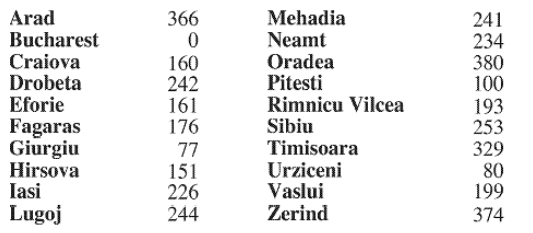
\includegraphics[width=0.75\textwidth]{images/esempio-euristica-h.png}
    \end{figure}
\end{example}

\subsection{Algoritmo di ricerca Best-first}
Il \textbf{best first - heuristic} usa lo stesso algoritmo di UC \footnote{Warning: AIMA ed. IV ha usato uno schema di
UC diverso e alcune proprietà cambiano} ma con uso di $f$ (stima di costo) per la coda con priorità.
Una volta scelta $f$ determina la strategia di ricerca. A ogni passo si sceglie il nodo sulla frontiera per cui il valore della $f$ è 
migliore (il nodo più promettente).
\begin{note}
    Migliore significa "minore" in caso di un'euristica che stima la distanza della soluzione
\end{note}
\hspace{-15pt}Un caso speciale: \textbf{greedy best-first}, su usa solo $h (f=h)$.
\begin{example}
    Esempio di greedy best-first con $f=h$
    \begin{figure}[h!]
        \centering
        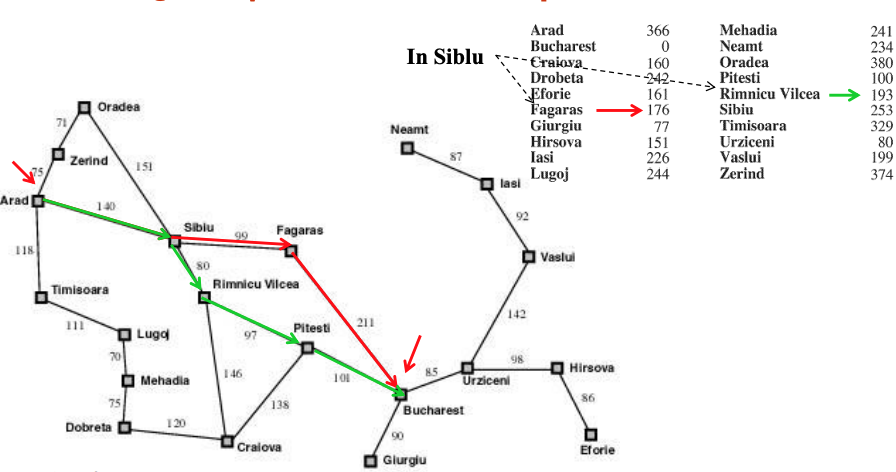
\includegraphics[width=0.75\textwidth]{images/esempio-best-first.png}
    \end{figure}
    Da Arad a Bucarest con \textbf{Greedy best-first}: Arad, sibiu, fagaras, bucharest (450) ma non è l'ottimale
    che sarebbe: Arad, Sibiu, Rimnicu, Pitesti, Bucarest (418).
\end{example}

\subsection{Algoritmo A}
Si può dire qualcosa di $f$ per avere garanzie di completezza e ottmialità?
\begin{definition}
    Un \textbf{Algoritmo A} è un algoritmo di best first con una fuzine di valutazione dello stato del tipo:
    $$f(n) = g(n) + h(n) \:\: \text{con}\:\: h(n) \geq 0 \:\: \text{e}\:\: h(goal) = 0$$
\end{definition}
In questa definizione abbiamo che $g(n)$ è il costo del cammino percorso per raggiugnere n, mentre $h(n)$ una
stima del costo per raggiungere da n un nodo goal (distanza).\\
Vedremo alcuni casi particolari dell'algoritmo A:
\begin{itemize}
    \item Se $h(n) = 0 \:\:[f(n) = g(n)]$ si ha \textbf{Ricerca Uniforme (UC)}.
    \item Se $g(n) = 0 \:\:[f(n) = h(n)]$ si ha \textbf{Greedy Best First}.
\end{itemize}
\begin{example}
    Esempio nel gioco dell'otto.
    \begin{figure}[h!]
        \centering
        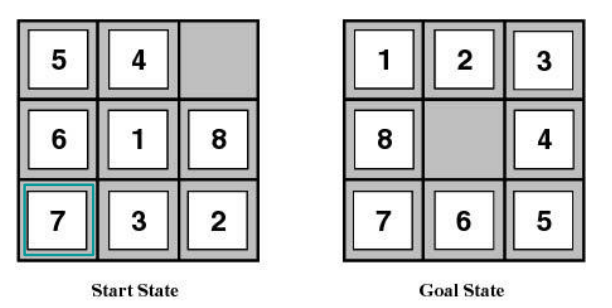
\includegraphics[width=0.6\textwidth]{images/esempio-gioco-otto.png}
    \end{figure}

    \hspace{-15pt}$f(n) = \#\text{mosse fatte} \:\: + \:\: \#\text{caselle-fuori-posto} \hspace{10pt} f(start) = 0 + 7 \hspace{10pt} f(goal-state) = ? + 0$\\
    Dopo $\leftarrow, \downarrow, \uparrow, \rightarrow$ abbiamo che $f = 4 + 7$, stesso stato, $g$ è cambiato.
\end{example}
\begin{theorem}
    L'algoritmo A con la condizione:
    $$g(n) \geq d(n) \cdot \epsilon \hspace{10pt}(\epsilon >0 \text{ costo minimo arco})$$
    è completo (con $d(n)$ che è la distanza).
\end{theorem}
\begin{note}
    La conzione ci garantisce che non si verifichino situazioni strane del tipo:
    \begin{figure}[h!]
        \centering
        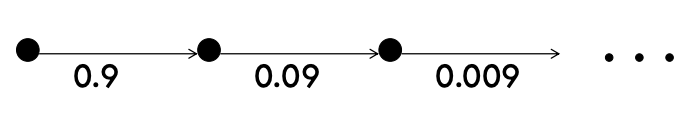
\includegraphics[width=0.65\textwidth]{images/nota-alg-completo.png}
    \end{figure}
    e quindi che il costo lungo un cammino non cresca "abbastanza" (se cresce abbastanza possiamo fermare quel path per costo alto di g).
\end{note}
\begin{demostration}
    Sia $[n_0, n_1, n_2, \dots, n', \dots, n_k = goal]$ un cammino soluzione. Sia $n'$ un nodo della frontiera su un cammino soluzione:
    $n'$ prima o poi sarà espanso. Infatti esistono solo un numero finito di nodi $x$ che possono essere aggiunti alla frontiera con $f(x) \leq f(n')$
    (è la condizione sulla crescita di g, scritta precedentemetne, tale che non esista una catena infinita di archi e nodi che possa aggiungere con costo sempre $\leq f(n')$).\\\\
    Quindi, se non si trova una soluzione prima, $n'$ verrà espanso e i suoi successori aggiunti alla frontiera. Tra questi anche il suo successore sul cammino soluzione.\\
    Il ragionamento si può ripetere fino a dimostrare che anche il nodo goal sarà selezionato per l'espanzione.
\end{demostration}

\subsection{Algoritmo $A^*$}
La funzione di valutazione ideale (oracolo):
$$f^*(n) = g^*(n) + h^*(n)$$
Con $g^*(n)$ il costo del cammino minimo da radice a n, $h^*(n)$ costo del cammino minimo da n a goal, $f^*(n)$ costo
del cammino minimo da radice a goal, attraverso n. Normalmente:
$$g(n) \geq g^*(n) \hspace{10pt} e \hspace{10pt} h(n) \text{ è una stima di } h^*(n)$$
($g(n) \geq g^*(n)$ rappresenta costo cammino $\geq$ costo migliore). Si può andare in sottostima (e.g. linea d'aria) o 
sovrastima della distanza dalla soluzione.
\begin{definition}[Euristica ammissibile]
    $$\forall n\:\: t.c.\:\: h(n) \leq h^*(n) \:\:\:\: \text{h è una sottostima}$$
\end{definition}
\begin{example}
    L'euristica della distanza in linea d'aria.
\end{example}
\begin{definition}[Algoritmo $A^*$]
    Un algoritmo A in cui h è una funzione euristica ammissibile.
\end{definition}
\begin{theorem}
    Gli algoritmi $A^*$ sono \textbf{ottimali}.
\end{theorem}
\begin{corollaries}
    $BF^{(+)}$ e UC sono ottimali ($h(n) = 0$).
\end{corollaries}
\begin{example}
    Itinerario con $A^*$ (ad albero).
    \begin{figure}[h!]
        \centering
        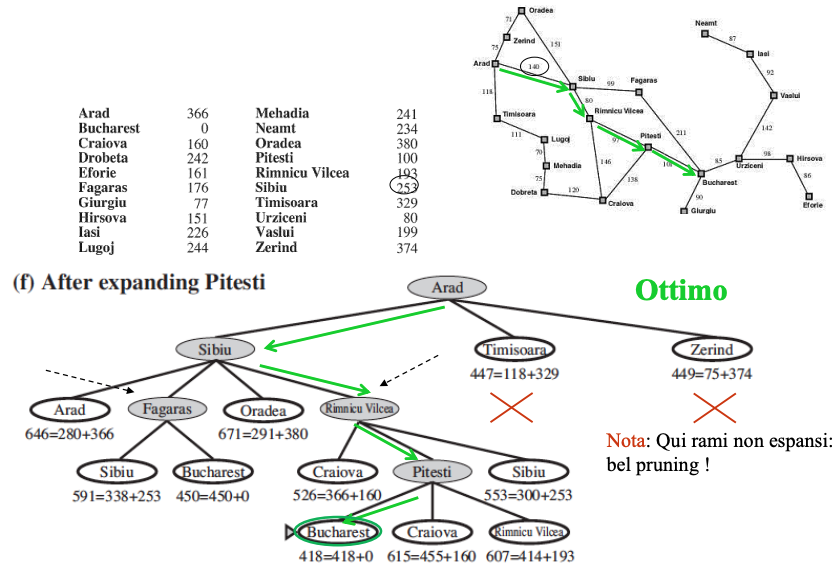
\includegraphics[width=0.62\textwidth]{images/itinerario-A*-albero.png}
    \end{figure}
\end{example}
\begin{observation}
    Alcune osservazioni su $A^*$
    \begin{enumerate}
        \item Rispetto a greedy best-first, la componente g fa si che si abbandonino cammini che vanno troppo in profondità.
        \item Ha sotto o sovra stima?
        \begin{enumerate}
            \item Una sottostima (h) può farci compiere del lavoro inutile (tenendo anche candidati non buoni), però non ci 
            fa perdere il cammino migliore (quando prendo nodo goal è il cammino migliore).
            \item Una funzione che qualche volta sovrastima può farci perdere la soluzione ottimale (taglio per causa di sovrastima, invece era buona)
        \end{enumerate}
    \end{enumerate}
\end{observation}

\subsubsection{Ottimalità su $A^*$}
\begin{wrapfigure}[8]{r}{5cm}
    \vspace{-30pt}
    \centering
    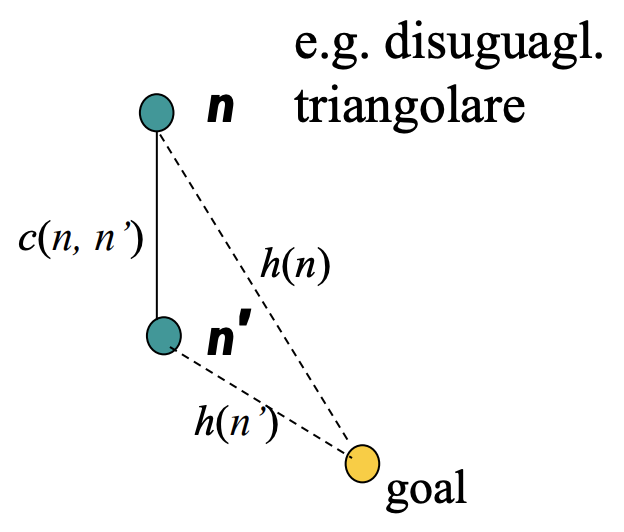
\includegraphics[width=4cm]{images/dis-triagolare.png}
\end{wrapfigure}
Nel caso di ricerca a/su albero l'uso di un'euristica ammissibile è sufficente a garantire l'ottimalità su $A^*$.
Nel caso di ricerca su grafo (con UC come visto) serve una proprietà più forte: la \textbf{consistenza} (detta anche \textbf{monotonicità}).\\\\
Per evitare rischio di scartare candidati ottimi (stato già incontrato) si vuol evitare, causa uso della lista esplorati, di far sparire, o meglio
non considerare al momento dell'espansione, candidati ottimali. Cerchiamo quindi condizioni per garantire che il primo espanso sia il migliore.

\begin{definition} 
    Un euristica \textbf{consistente} $[h(goal) = 0]$ (consistenza locale).
    $$\forall n \:\: t.c. \:\: h(n) \leq c(n, a, n') + h(n') \text{ dove n' è un successore di n}$$
\end{definition}
\hspace{-15pt}Ne segue che $f(n) \leq f(n')$
\begin{note}
    Se h è consistente la $f$ non decresce mai lungo i cammini, da cui il termine \textbf{monotona}.
\end{note}
\begin{theorem}
    Un'euristica monotona è ammissibile.
\end{theorem}
\hspace{-15pt}Esistono euristiche ammissibili che non sono monotone, ma sono rare. Le euristiche monotone garantiscino che la soluzione meno costosa 
venga trovata per rima e quindi sono ottimali anche nel caso di ricerca su grafo.\\
Non si devono recuperare tra gli antenati nodi con costo minore. Lista degli esplorati, stato già esplorato è sul cammino ottimo allora posso
evitare di inserire il corrente ripetuto senza perdere l'ottimalità.
\begin{lstlisting}
    if figlio.Stato non e in esplorati e non e in frontiera then
        frontiera = Inserisci(figlio, frontiera)
\end{lstlisting}
Per la frontiera, volendo evitare stati ripetuti, resta 'if' finale di UC:
\begin{lstlisting}
    if figlio.Stato e in frontiera con Costo-cammino piu alto then
        sostituisci quel nodo frontiera con figlio 
\end{lstlisting}
Andiamo ora a verificare l'ottimalità di $A^*$ supponendo di avere il teorema, con $h$ consistente.
\begin{enumerate}
    \item Se $h(n)$ è consistente i valori di $f(n)$ lungo un cammino sono non decrescenti:
    $$\text{se } h(n) \leq c(n, a, n') + h(n') \hspace{10pt} \Rightarrow \text{(def. consistenza sommando g(n))}\hspace{10pt} g(n) + h(n) \leq g(n) + c(n, a, n') + h(n')$$
    ma siccome abbiamo $g(n) + c(n, a, n') = g(n')$ allora
    $$g(n) + h(n) \leq g(n') + h(n') \Rightarrow f(n) \leq f(n') \Rightarrow f \text{ monotona}$$
    \item Ogni volta che $A^*$ seleziona un nodo (n) per l'espansione, il cammino ottimo a tale nodo è stato trovato: 
    se così non fosse, ci sarebbe un altro nodo m ella frontiera sul cammino ottimo (a n, ancora da trovare con un cammino ottimo), con $f(m)$
    minore (per la monotonia e n successore di m); ma ciò non è possibile perché tale nodo sarebbe già stato espanso (si espande prima un nodo con f minore).
    \item Quando seleziona nodo goal è cammino ottimo $[h=0, f=C^*]$.
\end{enumerate}
% TODO: AGGIUNGI IMMAGINI
Quindi, detto questo, perché $A^*$ è vantaggioso?
\begin{itemize}
    \item $A^*$ espande tutti i nodi con $f(n) < C^*$ ($C^*$ = costo ottimo)
    \item $A^*$ espande alcuni nodi con $f(n) = C^*$.
    \item \textbf{$A^*$ non espande alcun nodo con $f(n) > C^*$}
\end{itemize}
Quindi alcuni nodi (e suoi sottoalberi) non verranno considerati per l’ espansione (ma restiamo ottimali):
pruning (h opportuna, più alta possibile tra le ammissibili, fa tagliare molto).\\\\
% TODO: AGGIUNGI IMMAGINE
Più f è aderente a stima ottimale, più taglio! Ovali più stretti. Cercheremo quindi una h il più alta possibile tra le ammissibili
Se molto bassa molti (sino a tutti i) nodi restano minore di $C^* \to$ espando tutti (a cerchi).
Il pruning sotto-alberi è il punto focale: non li abbiamo già in memoria e evitiamo di generarli (decisivo per i problemi di AI a spazio stati esponenziali.\\\\
In riassunto L’algoritmo è quello degli schemi usati per UC, Usando f = g+h per la coda con priorità, ove h e g soddisfano quanto allo slide 9 [A], 
ove h è una funzione euristica ammissibile $[A^*]$, e considerando le condizioni dette per ottenere l’ottimalità su grafi.
\begin{itemize}
    \item $A^*$ è \textbf{completo}: discende dalla completezza di A ($A^*$ è un algoritmo A particolare).
    \item $A^*$ con euristica monotona è \textbf{ottimale}.
    \item $A^*$ è \textbf{ottimamente efficiente}: a parità di euristica nessn altro algoritmo espande meno nodi (senza rinunciare a ottimalità)
\end{itemize}
I problemi principali sono la scelta dell'euristica e  ancora l'occupazione di memoria che nel caso
pessimo resta esponenziale come visto per gli altri algoritmi di ricerca con stesso schema, causa frontiera.

\subsection{Sotto-casi speciali: US e Greedy Best First}
Ci sono due casi particolai dell'algoritmo A:
\begin{enumerate}
    \item Se $h(n) = 0$ $[f(n) = g(n)]$ si ha Uniform Cost (UC), ossia $g$ non basta (si può migliorare).
    \item Se $g(n) = 0$ $[f(n) = h(n)]$ si ha Greedy Best Fist, ossia $h$ non basta (già visto all'inizio).
\end{enumerate}
\subsubsection{UC vs $A^*$}
Illustrazione dell'algoritmo di ricerca Dijkstra per trovare il percorso da un nodo iniziale (in basso
sinistra, rosso) a un nodo obiettivo (in alto a destra, verde) in un problema di pianificazione del movimento del robot.
I nodi aperti rappresentano l'insieme "provvisorio". I nodi pieni sono quelli visitati, con colore
che rappresenta la distanza: più verde, più lontano. Nodi in tutti i diversi
le direzioni vengono esplorate in modo uniforme, apparendo come un fronte d'onda più o meno circolare
poiché l'algoritmo di Dijkstra utilizza un'\textbf{euristica identicamente uguale a 0}. $\to$ UC !\\\\
\begin{wrapfigure}[6]{r}{5cm}
    \vspace{-35pt}
    \centering
    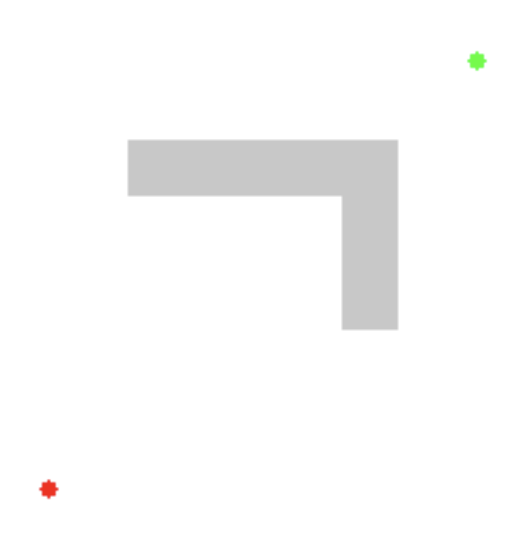
\includegraphics[width=3cm]{images/dijkstra.png}
\end{wrapfigure}
Illustrazione dell'algoritmo di ricerca A* per trovare il percorso da un nodo iniziale a un nodo obiettivo in un robot è un
problema di pianificazione del movimento. I cerchi vuoti rappresentano i nodi nell'insieme aperto, cioè,
quelli che restano da esplorare e quelli pieni sono nell'insieme chiuso. Colore acceso
ogni nodo chiuso indica la distanza dalla partenza: più è verde, più è lontano. Uno
può prima vedere A* muoversi in linea retta in direzione della porta, poi quando colpisce l'ostacolo, esplora percorsi alternativi attraverso i nodi da insieme aperto $\to$ frontiera.\\\\
L'algoritmo A* è una generalizzazione dell'algoritmo di Dijkstra che riduce le dimensioni del sottografo che deve essere esplorato, se il lower-bound
della "distanza" dall'obiettivo (h) è disponibile.

\subsection{Costruire le euristiche di $A^*$}
Partiamo dalle valutazione di funzioni euristiche. A parità di ammissibilità, una euristica può essere più
efficiente di un’altra nel trovare il cammino soluzione migliore (visitare meno nodi). Questo dipende da quanto
informata è l'euristia (dal \textbf{grado di informazione posseduto}) 
\begin{itemize}
    \item $h(n) = 0$ minimo di informazione (BF o UC)
    \item $h^*(n)$ massimo di infomrazione (oracolo)
\end{itemize}
In generale, per le euristiche ammissibili:
$$0 \leq h(n) \leq h^*(n)$$
\begin{theorem}
    Se $h_1 \leq h_2$, i nodi espansi\footnote{Ricorda che $A^*$ espande tutti i nodi con $f(n) = g(n) + h(n) < C^*$, e sono meno per $h$ maggiore (h maggiore fa andare più nodi oltre $C^*$).} da $A^*$ con $h_2$ sono un sottoinsieme di quelli espandi da $A^*$ con $h_1$.
\end{theorem}
\hspace{-15pt}Se $h_1 \leq h_2$, $A^*$ con $h_2$ è almeno efficiente quanto $A^*$ con $h_1$.
Un’euristica più informata (accurata) riduce lo spazio di ricerca (è più efficiente), ma è tipicamente più costosa da calcolare (e.g. un caso estremo ?)
\begin{example}
    Due euristiche ammissibili per il gioco dell'8 potrebbero essere le seguenti:
    \begin{itemize}
        \item $h_1$: conta il numero di caselle fuori posto
        \item $h_2$: somma delle distanze \textbf{Manhattan} (orizzonatle/verticale) delle caselle fuori posto dalla posizione finale.
    \end{itemize}
    $h_2$ è più informata di $h_1$, infatti $\forall n \:\:.\:\: h_1(n) \leq h_2(n)$, quindi si dice che $h_2$ \textbf{domina} $h_1$ (utile per confrontte tra ammissibili)
    \begin{figure}[h!]
        \centering
        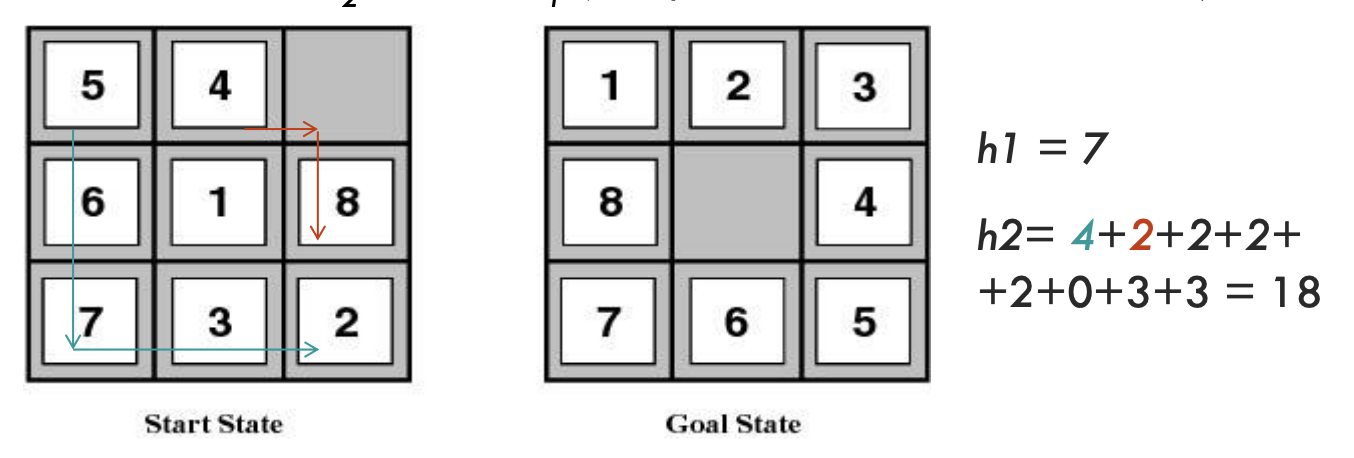
\includegraphics[width=0.65\textwidth]{images/euristica-gioco-8.png}
    \end{figure}
\end{example}
\begin{definition}
    La somma delle distanze Manghattan si definisce come:
    $$h((x,y)) = MD((x,y), (x_g, y_g)) = |x - x_g| + |y - y_g|$$
\end{definition}
\begin{figure}[h!]
    \centering
    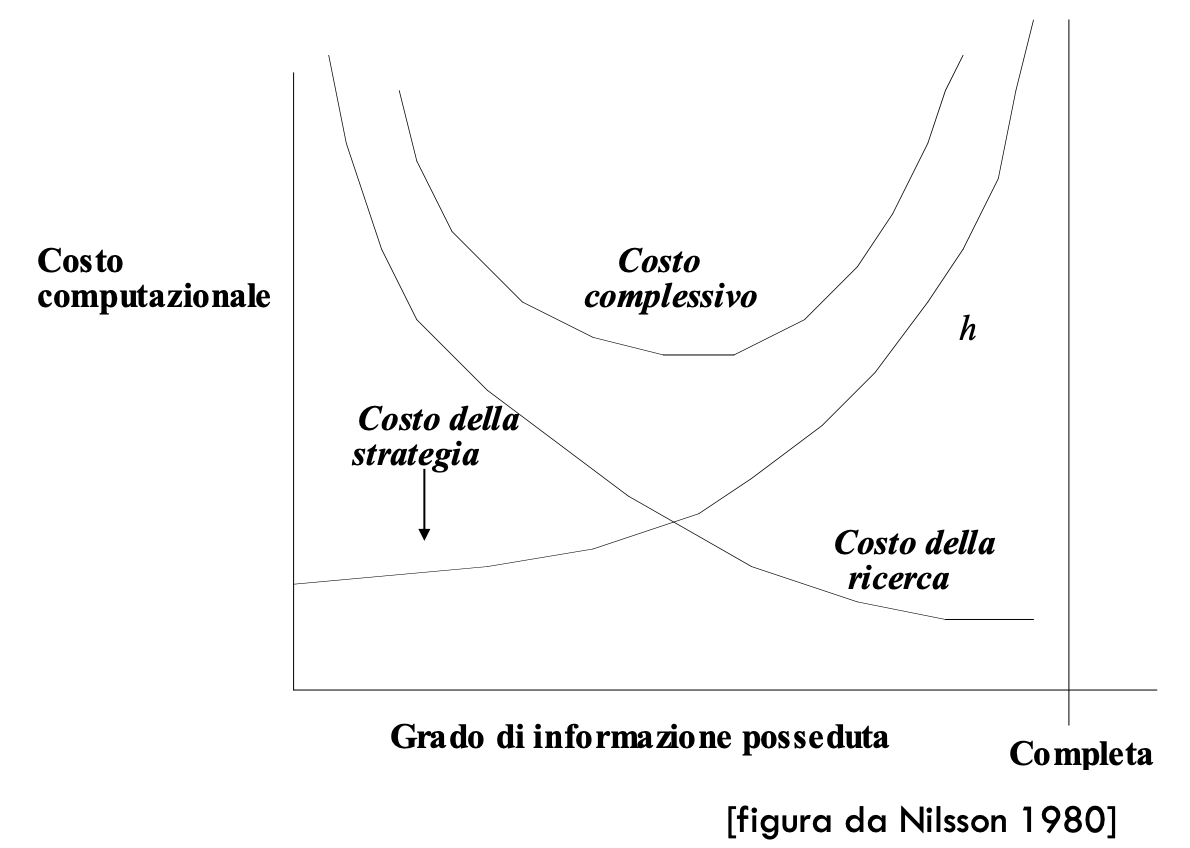
\includegraphics[width=0.60\textwidth]{images/costo-ricerva-vs-costo-euristica.png}
    \caption{Costo ricerca vs costo euristico}
\end{figure}
\hspace{-15pt}Ora capiamo come valutare gli algoritmi di ricerca euristica. Introfuciamo
il \textbf{fattore di diramazione effettivo} $b^*$, N: numero di nodi generati, d: profondità della soluzione.
$b^*$ è il fattore di diramazione di un albero uniforme con $N+1$ nodi, solizione dell'equazione:
$$N + 1 = b^* + (b^*)^2 + \dots + (b^*)^d$$
Sperimentalmente una buona euristica ha un $b^*$ abbastanza vicino a 1 (<1.5)
\begin{example}
    Ricodando l'esempio dal gioco dell'otto:
    \begin{figure}[h!]
        \centering
        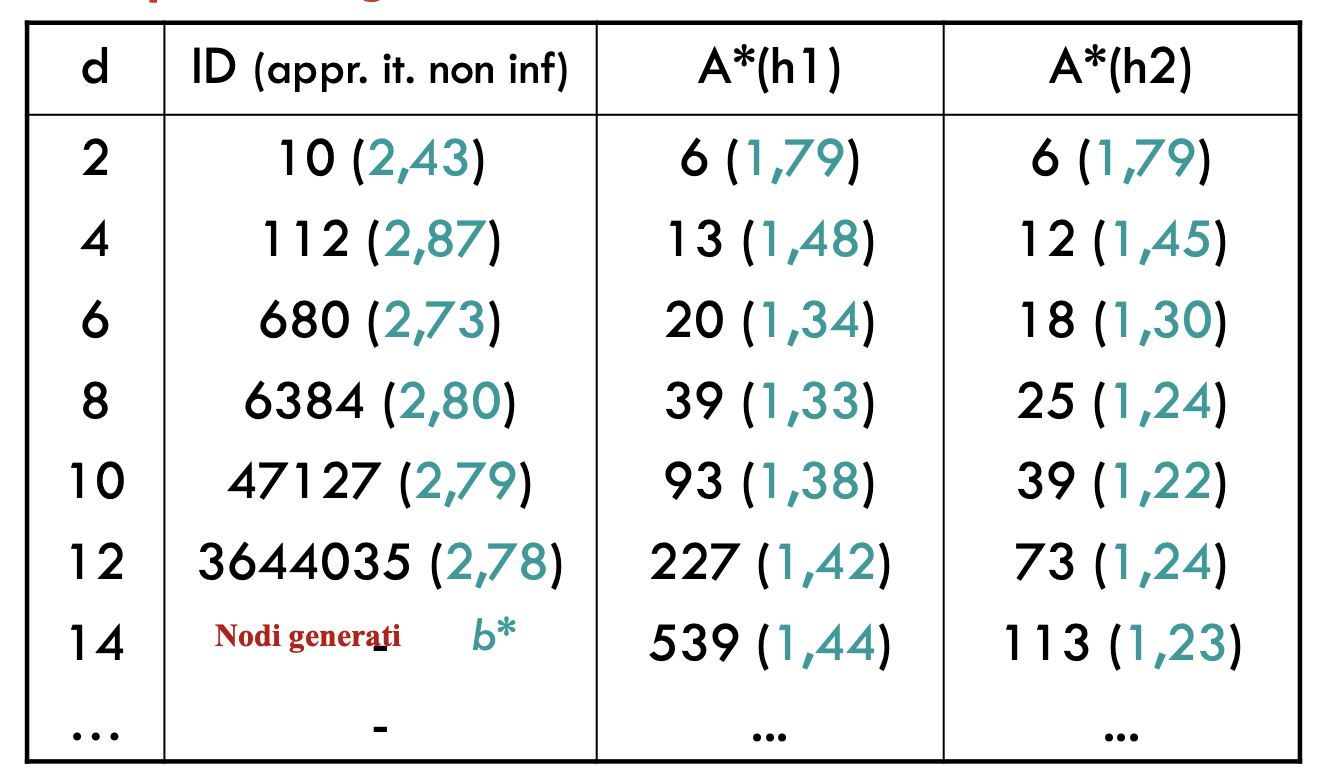
\includegraphics[width=0.60\textwidth]{images/gioco-otto-misura-euristiche.png}
    \end{figure}
    Sono riportati: Nodi generati e fattore di diramazione effettivo ($b^*$, verde)
    I dati sono mediati, per ogni d, su 100 istanze del problema [AIMA].\\\\
    Nella \textbf{capacità di esplorazione}, l'influenza di $b^*$:
    \begin{itemize}
        \item Con b=2: d=6 e N = 100 \hspace{15pt} d=12 e N = 10.0000
        \item Con b=1.5: d=12 N = 100 \hspace{15pt} d=24 e N = 10.000
    \end{itemize}
    migliorando di poco l’euristica si riesce, a parità di nodi espansi, a raggiungere una profondità doppia di esplorazione mosse!
\end{example}

\subsection{Inventare euristiche}
Quindi abbiamo che:
\begin{enumerate}
    \item Tutti i problemi dell’IA (o quasi) sono di complessità esponenziale ... (nel generare nodi, i.e. configurazioni possibili) ma c’è esponenziale e esponenziale!
    \item L’euristica può migliorare di molto la capacità di esplorazione dello spazio degli stati rispetto alla ricerca cieca.
    \item Migliorando anche di poco l’euristica si riesce ad esplorare uno spazio molto più grande (più in profondità).
\end{enumerate}
Per inventare un euristica ci sono alcune strategie, che aiutano appunto ad ottenre euristiche amissibili:
\begin{itemize}
    \item Rilassamento del problema
    \item Massimizzazione di euristiche
    \item Database di pattern disgiunti
    \item Combinazione lineare
    \item Apprendere dall’esperienza
\end{itemize} 
\subsubsection{Rillassamento problema}
\begin{example}
    Il rilassamento del problema nel gioco dell’8 mossa da A a B possibile se: 
    \begin{enumerate}
        \item \textbf{B adiacente a A}
        \item \textbf{B libera}
    \end{enumerate}
    $h_1$ e $h_2$ sono calcoli distanza esatta della soluzione in versioni semplificate del puzzle:
    \begin{itemize}
        \item $h_1$ (nessuna restrizione, ne 1 ne 2): sono sempre ammessi scambi a piacimento tra caselle (si muove
        ovunque) $\to$ numero caselle fuori posto.
        \item  $h_2$ (solo restrizione 1): sono ammessi spostamenti anche su caselle occupate, purché adiacenti $\to$ somma delle distanze Manhattan.
    \end{itemize}
\end{example}

\subsubsection{Massimizzazione di euristiche}
Se si hanno una serie di euristiche ammissibili $h_1, h_2, \dots, h_k$ \textbf{senza che nessuna "domini" un'altra}
allora conviene prendere il massimo dei lori valori:
$$h(n) = max(h_1(n), h_2(n), \dots, h_k(n))$$
Se le $h_i$ sono ammissibili, anche la $h$ lo è. La h domina tutte le altre.

\subsubsection{Database con pattern disgiunti}
\begin{figure}[h!]
    \centering
    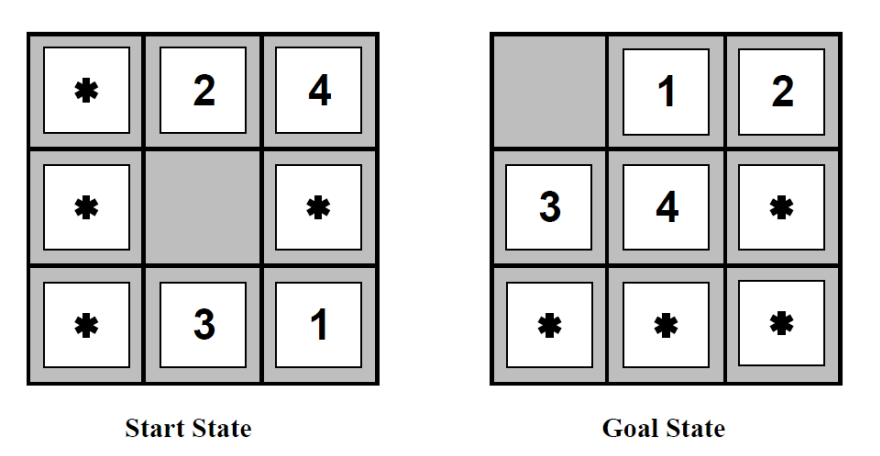
\includegraphics[width=0.65\textwidth]{images/euristiche-da-sottoproblemi.png}
\end{figure}
\hspace{-15pt}Costo della soluzione ottima al sottoproblema (di sistemare 1,2,3,4) è una sottostima del costo per il problema nel suo
complesso (e.g. rilevatesi più accurata della Manhattan). \\
\textbf{Database di pattern}: memorizzare ogni istanza del
sottoproblema con relativo costo della soluzione. Usare poi questo database per calcolare $h_{DB}$ (estraendo dal DB la
configurazione corrispondente allo stato completo corrente).
\begin{itemize}
    \item \textbf{Domanda}: Potremmo poi fare la stessa cosa per altri sottoproblemi: 5-6-7-8, 2-4-6-8, ottenendo altre euristiche ammissibili,
    poi prendere il valore massimo: ancora una euristica ammissibile. Ma potremmo sommarle e ottenere un’euristica
    ancora più accurata?
    \item \textbf{Risposta}: In generale no perché le soluzioni ai sottoproblemi interferiscono (condividono alcune mosse, se sposto 1-2-3-4, spostero
    anche 4-5-6-7) e la somma delle euristiche in generale non è ammissibile (potremmo sovrastimare avendo avuto aiuti mutui).
    Si deve eliminare il costo delle mosse che contribuiscono all’altro sottoproblema. Database di pattern disgiunti consentono di sommare i
    costi (euristiche additive) [e.g. solo costo mosse su1-2-3-4], sono molto efficaci: gioco del 15 in pochi ms
    ma per esempio difficile scomporre per cubo Rubik.
\end{itemize}

\subsubsection{Apprendimento dall'esperienza}
Bisogna eseguire un apprendimento dall'esperienza. Quindi far girare il programma, raccogliere dati: coppie
$<stato, h^*>$. Usare i dati per apprendere a predire la h con algoritmi di apprendimento induttivo (da istanze note stimiamo h in generale).\\
Gli algoritmi di apprendimento si concentrano su caratteristiche salienti dello stato (feature, xi) [e.g.
apprendiamo che da numero tasselli fuori posto 5 $\to$ costo~14, etc].

\subsubsection{Combinazione euristiche}
Quando diverse caratteristiche influenzano la bontà di uno stato, si può usare una combinazione lineare per combinare le euristiche:
$$h(n) = c_1 x_1(n) + c_2x_2(n) + \dots + c_k x_k(n)$$
\begin{example}
    Gioco dell'8: $h(n) = c_1 \:\: \#\text{fuori-posto} + c_2 \#\text{coppie-scambiate}$\\
    Scacchi: $h(n) = c_1 \:\text{vant-pezzi} + c_2 \:\text{pezzi-attacc.} + c_3 \:\text{regina} + \dots$
\end{example}
\hspace{-15pt}Il peso dei coefficienti può essere aggiustato con l’esperienza, anche qui apprendendo automaticamente da esempi di gioco.
$h(goal) = 0$ (e.g. gioco dell’8) ma ammissibilità e consistenza non automatiche.

\subsection{Algoritmi evoluti basati su $A^*$}
Ci sono una serie di algoritmi basati su $A^*$ che possono andare a portare ad un miglioramento dell'occupazione della memoria.
Fra questi abbiamo: Beam search, A* con approfondimento iterativo (IDA*), ricerca best-first ricorsiva (RBFS), A* con memoria limitata (MA*) in versione semplice (SMA*).

\subsubsection{Beam search}
Nel Best First viene tenuta tutta la frontiera; se l’occupazione di memoria è eccessiva si può ricorrere ad una variante: la Beam search.
La Beam Search tiene ad ogni passo solo i k nodi più promettenti, dove k è detto l’ampiezza del raggio
(beam). La Beam Search non è completa.

\subsubsection{IDA${}^*$}
L'$IDA^*$ è un $A^*$ con approfondimento iterativo. IDA* combina A* con ID: ad ogni iterazione si ricerca
in profondità con un limite (cut-off) dato dal valore della funzione f (e non dalla profondità) il limite f-limit viene aumentato ad ogni iterazione,
fino a trovare la soluzione. Punto critico: di quanto viene aumentato f-limit.
\begin{example}
    \begin{figure}[h!]
        \centering
        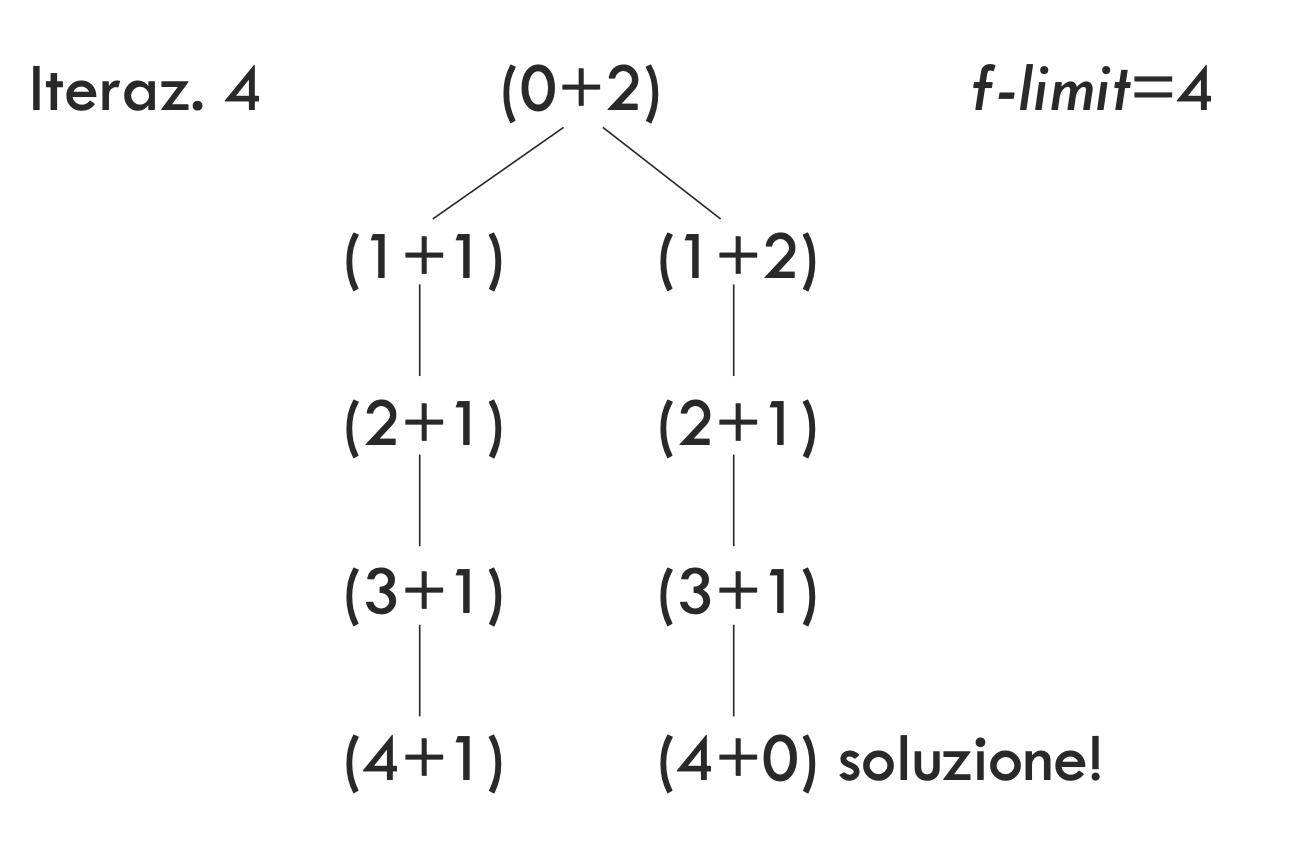
\includegraphics[width=0.65\textwidth]{images/esempio-ida*.png}
    \end{figure}
\end{example}
\hspace{-15pt}Cruciale la scelta dell'incremento per garantire l’ottimalità:
\begin{itemize}
    \item Nel caso di costo delle azioni fisso è chiaro: il limite viene incrementato del costo delle azioni.
    \item Nel caso che i costi delle azioni siano variabili? O costo minimo, oppure si potrebbe ad ogni passo fissare il limite successivo al
    valore minimo delle f scartate (in quanto superavano il limite) all’iterazione precedente.
\end{itemize}
$IDA^*$ è sia completo che ottimale.
\begin{itemize}
    \item Se le azioni hanno costo costante k (caso tipico 1) e f-limit viene incrementato di k.
    \item Se le azioni hanno costo variabile e l'incremento di f-limit è $\leq \epsilon$ (minimo costo degli archi).
    \item Se il nuovo f-limit = min. valore f dei nodi generati ed esclusi all'iterazione precedente.
\end{itemize}
L'occupazione di memoria è $O(bd)$.

\subsubsection{Best-first ricorsivo (BRFS)}
Simile a DF ricorsivo: cerca di usare meno memoria, facendo del lavoro in più. Tiene traccia ad ogni livello del \textbf{migliore percorso
alternativo}. Invece di fare backtracking in caso di fallimento (DF si ferma solo in fondo) interrompe l’esplorazione quando
trova un nodo meno promettente (secondo f). Nel tornare indietro si ricorda il miglior nodo che ha
trovato nel sottoalbero esplorato, per poterci eventualmente tornare Memoria: lineare nella profondita delle sol. ottima.
\begin{example}
    \begin{figure}[h!]
        \centering
        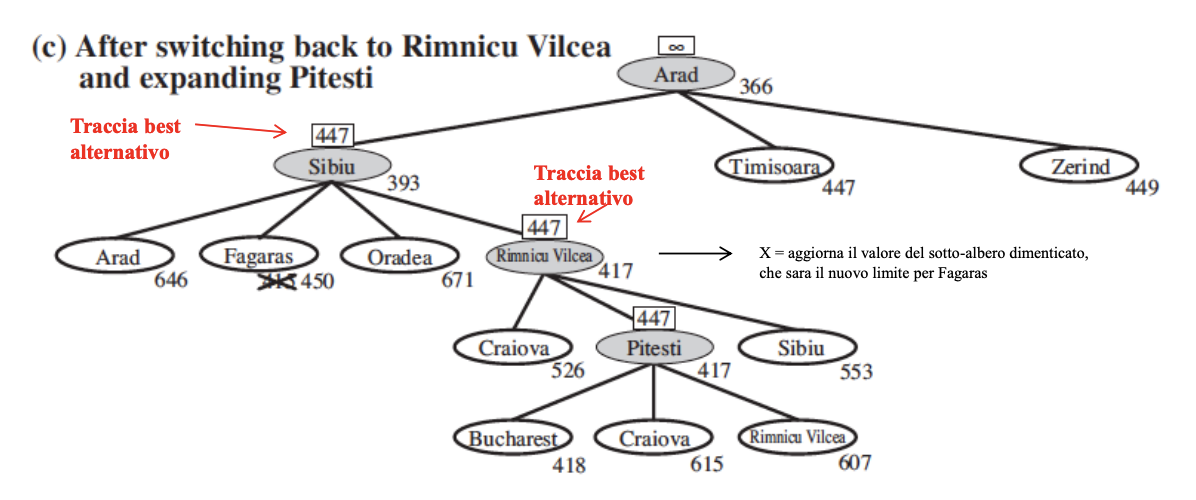
\includegraphics[width=0.65\textwidth]{images/esempio-best-first-ricorsivo.png}
    \end{figure}
\end{example}
\begin{lstlisting}
    function Ricerca-Best-First-Ricorsiva(problema)
        returns soluzione oppure fallimento
        // all inizio f-limite e un valore molto grande
        return RBFS(problema, CreaNodo(problema.Stato-iniziale), infinito) 

    function RBFS (problema, nodo, f-limite)
        // restituisce due valori
        returns soluzione oppure fallimento e un nuovo limite all f-costo 
        if problema.TestObiettivo(nodo.Stato) then return Soluzione(nodo)
        successori = [ ]

        for each azione in problema.Azioni(nodo.Stato) do
            aggiungi Nodo-Figlio(problema, nodo, azione) a successori // genera i successori
        if successori vuoto then return fallimento, infinito

        for each s in successori do // valuta i successori
            s.f = max(s.g + s.h, nodo.f) // un modo per rendere monotona f
        loop do
            migliore = il nodo con f minimo tra i successori
            if migliore.f > f_limite then return fallimento, migliore.f
            alternativa = il secondo nodo con f minimo tra i successori
            risultato, migliore.f = RBFS(problema, migliore, min(f_limite, alternativa))
            if risultato != fallimento then return risultato
\end{lstlisting}

\subsubsection{$A^*$ con memoria limitata (versione semplice)}
L'idea è quella di utilizzare al meglio la memoria disponibile. $SMA^*$ procede come $A^*$ fino ad esaurimento della
memoria disponibile. A questo punto \textbf{“dimentica” il nodo peggiore}, dopo avere aggiornato il valore del padre.
A parità di f si sceglie il nodo migliore più recente e si dimentica il nodo peggiore più vecchio. Ottimale se il cammino soluzione sta in memoria.\\\\
In conclusione in algoritmi a memoria limitata (IDA* e SMA*) le limitazioni della memoria possono portare a compiere
molto lavoro inutile [esp. ripetuta stessi nodi]. Difficile stimare la complessità temporale effettiva. Le limitazioni di memoria possono rendere un problema intrattabile dal punto di vista computazionale.